\section{Introduction}

The main goal of this laboratory assignment is to analyse a RC circuit with sinusoidal excitation both theoretically and computationally, by simulating the circuit using \textit{Ngspice}. Throughout the theoretical analysis, the circuit will be essentially analysed using some methods and concepts such as the nodal analysis method and the Thévenin equivalent circuit or solving some differential equations to find the capacitor's natural response and the total solution of the system. \\

All the results and plots obtained in the theoretical analysis will be compared to the values and similar plots obtained by the simulation made in \textit{Ngspice} and discussed. \\

The analysed circuit was a RC circuit which can be seen in Fig. \ref{fig:bigscheme}.

\begin{figure}[H]
    \centering
    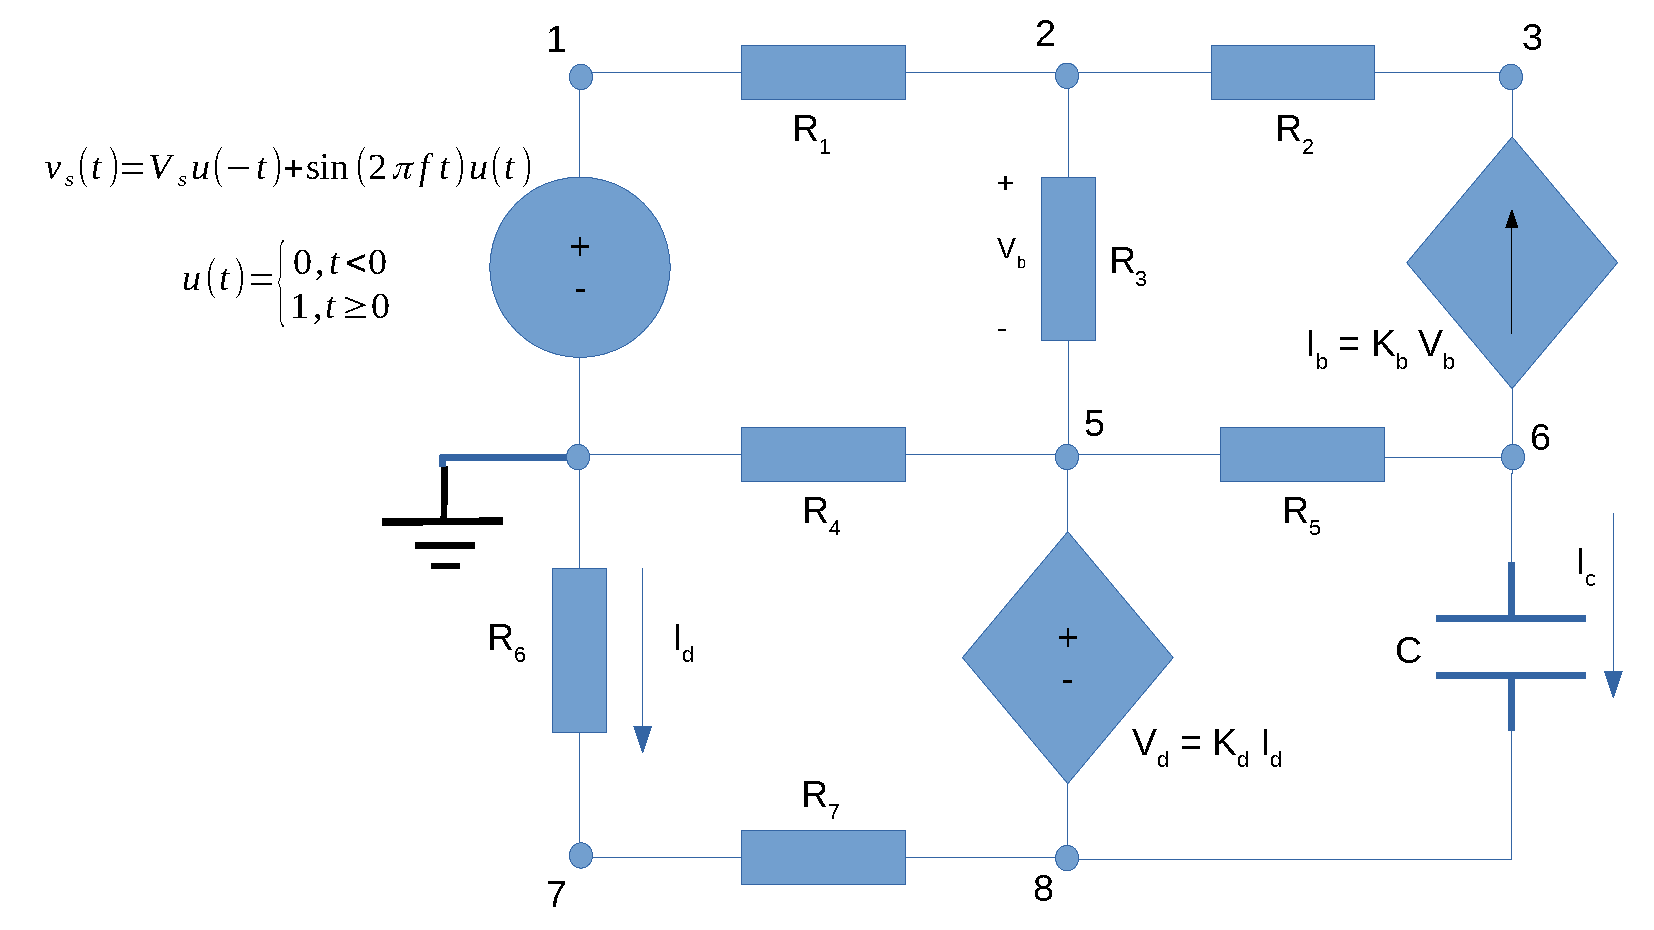
\includegraphics[width = 0.85\linewidth]{generalscheme.pdf}
        \caption{\textit{Circuit analysed. It consists, essentially, in a circuit with 4 meshes, 8 nodes and 11 branches (in which we count 7 resistors, 2 voltage sources - one of them controlled by the current $I_d$ - and 2 current sources - one independent and one dependent, controlled by the voltage $V_b$ as it can be seen in the figure). The labels used in this figure will be used throughout this report.}}
    \label{fig:bigscheme}
\end{figure}

As a starting point to this laboratory assignment, some values of the symbolic variables presented in Fig. \ref{fig:bigscheme} were given and are presented in Table \ref{tab:initial_values}:

\begin{table}[H]
    \begin{minipage}{.5\textwidth}
      \centering
      \begin{tabular}{c|c}
        \hline
        \multicolumn{2}{c}{Resistors [$k\Omega$]}  \\
        \hline
        $R_1$ & 1.03994439216 \\
        $R_2$ & 2.07923431764 \\
        $R_3$ & 3.06168544529 \\
        $R_4$ & 4.09516986362 \\
        $R_5$ & 3.00136467001 \\
        $R_6$ & 2.03324628446 \\
        $R_7$ & 1.02216788331
      \end{tabular}
    \end{minipage}
    \begin{minipage}{.5\textwidth}
      \centering
      \begin{tabular}{c|c}
        \hline
        \multicolumn{2}{c}{Capacitance [$\mu F$]}  \\
        \hline
        $C$ & 1.01674167773 \\
        \hline
        \hline
        \multicolumn{2}{c}{Voltages [$V$]}  \\
        \hline
        $V_s$ & 5.03847501972 \\
        \hline
        \hline
        \multicolumn{2}{c}{Dependent sources constants}  \\
        \hline
        $K_b$ & 7.01505323139 $mS$ \\
        $K_c$ & 8.37372457746 $k\Omega$
      \end{tabular}
    \end{minipage}
    \caption{Summary table with all the known values at the starting point}
    \label{tab:initial_values}
\end{table}